\section{Cell Growth}

% Task 2.1

% Simulate the growth of tumour cells for t=1200. Does the growth reach a steady state?
% If it has not, then experiment with the final time and determine the Time required to reach a steady state.

% 10 marks for basic simulation, 5 marks for showing time to reach final time 
% You can also use analytical methods to do the same

% Task 2.2

% Will the rate of growth reach a steady state or will the number increase as you keep increasing the size of the grid?
% What will happen if the value of M is changed - pick two values on either side of the value given.
% The issues associated with the numerical strategy you are employing,

% 5 marks for the part where you suggest what happens when the value of M changes, and why this is important


% Modelling the growth as a differential equation, we have the following equation:

% \[ \frac{dN}{dt}  = kNln\left(\frac{M}{n} \right) \]

% \[ N = \dfrac{M}{10^{4e^{-kt}}}  \]

Using the Euler method, we can simulate the differential equation for cell growth shown in \autoref{fig:task2-1}.
This uses the rate of growth at a point in time to calculate the number of cells at the next time step.

\setlength{\belowdisplayskip}{0pt} \setlength{\belowdisplayshortskip}{0pt}
\setlength{\abovedisplayskip}{0pt} \setlength{\abovedisplayshortskip}{0pt}

\begin{align*}
    M &= 10^{13} & k &= 0.06 & N &= 10^9 & 0 \leq t \leq 1200
\end{align*}

\begin{figure}[ht]
    \centering
    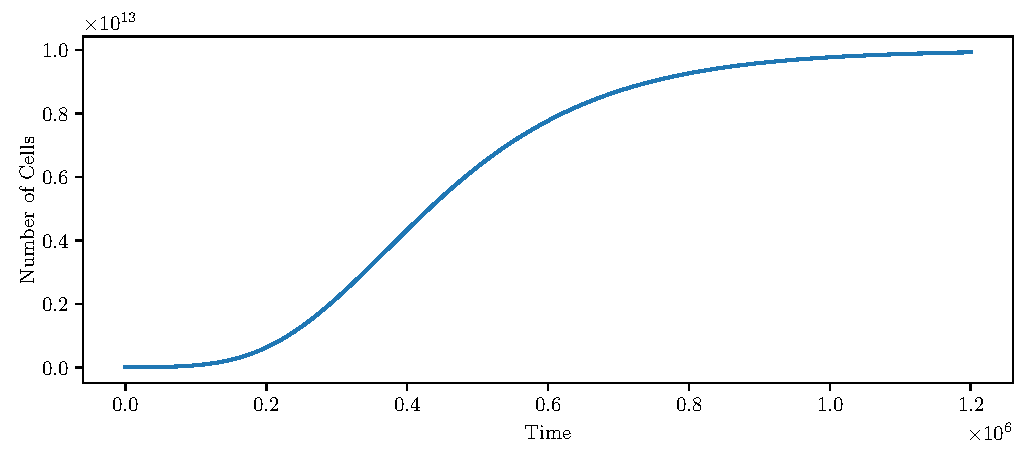
\includegraphics[width=14cm]{task2-1}
    \caption[Cell growth simulation]{Cell growth simulation}
    \label{fig:task2-1}
\end{figure}

The growth appears to reach a steady state at around 1200 time units, at this time the percentage of cells filled is 99.31\%.
Given the growth is modelled using an exponential function, the growth fills to 100\% at $t = \infty$,
this applies if the simulation has an infinite accuracy.
However on a computer system this value would be rounded up, resulting in a finite time to reach full capacity.
Steady state can be defined numerically as:

\begin{itemize}
    \item Percentage of cells filled is near 100\%.
    \item Rate of change of cell growth is near 0.
    \item Rate of change of the rate of change of cell growth is near 0.
\end{itemize}

\begin{figure}[ht]
    \centering
    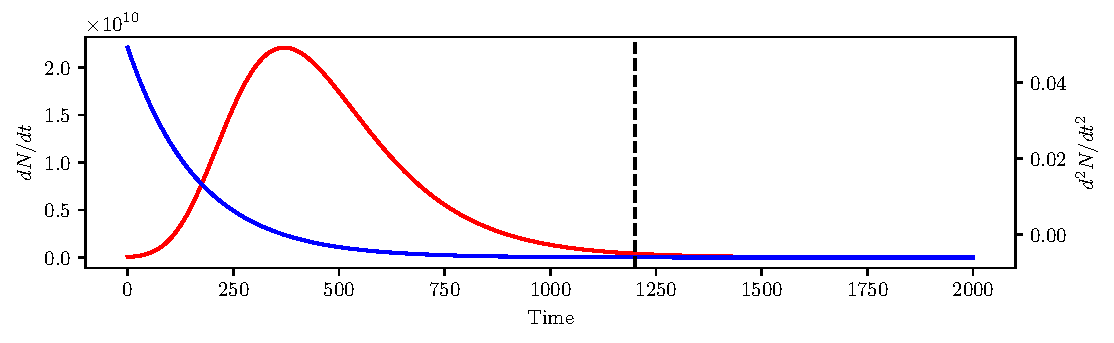
\includegraphics[width=14cm]{task2-1-t-dt}
    \caption[Cell growth simulation ($dN/dt$ and $d^2N/dt^2$)]{Cell growth simulation ($dN/dt$ and $d^2N/dt^2$)}
    \label{fig:task2-1-t-dt}
\end{figure}

% Graph displays both the rate of growth and the percentage of cells filled.

% \begin{figure}[ht]
%     \centering
%     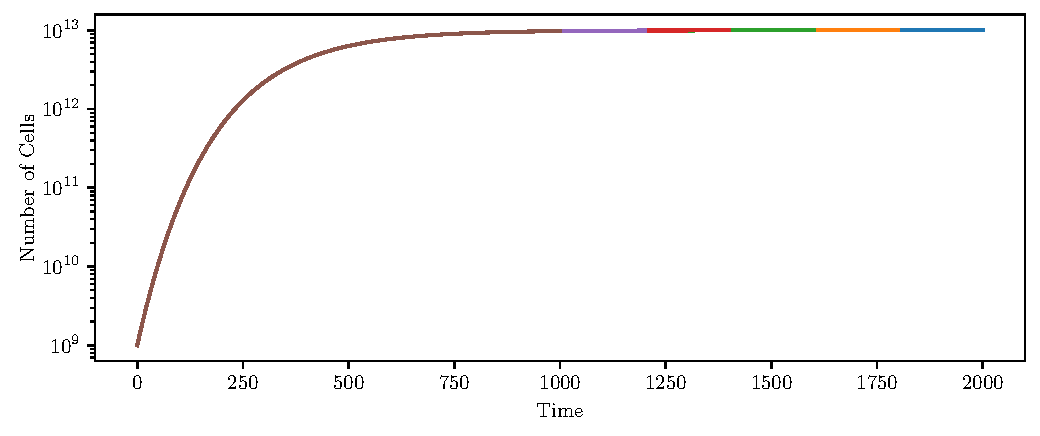
\includegraphics[width=14cm]{task2-1-t}
%     \caption[Cell growth simulation with different T values]{Cell growth simulation with different T values}
%     \label{fig:task2-1-t}
% \end{figure}

% \begin{center}
% \begin{tabular}{c | c c} 
%     T & Cells & \ Full \\
%     \hline
%     2000 & 1.00e+13 & 99.99\% \\
%     1800 & 1.00e+13 & 99.98\% \\
%     1600 & 9.99e+12 & 99.94\% \\
%     1400 & 9.98e+12 & 99.79\% \\
%     1200 & 9.93e+12 & 99.31\% \\
%     1000 & 9.77e+12 & 97.74\% \\    
% \end{tabular}
% \end{center}



% If the growth is modelled at a real value at t = infinity, the percentage of cells is 100\%.
% Anything less than infinity will have a percentage less than 100\%.

% Cannot simulate to infinity, so we have to simulate to a large enough value to reach a steady state.

% Analytically calculate the rate of growth for various values of T.

\autoref{fig:task2-1-t-dt} shows the rate of growth ($\frac{dN}{dt}$) and the rate of change of the rate of growth ($\frac{d^2N}{dt^2}$) for the simulation, solved analytically.
When we reach a value of $t = 1200$, the rate of growth is 4.083e+08, and the rate of change of the rate of growth is -0.005959.

\clearpage

\subsection{Accuracy of the Simulation}

% other differentiation methods...

When using the Euler method, the time step size ($h$ or $\Delta t$) is important for the accuracy of the simulation.
Larger values of $h$ will result in larger computation errors relative to the analytical solution.
\autoref{fig:task2-1-h} shows the growth  simulation with different values of $h$.

\begin{figure}[ht]
    \centering
    \begin{subfigure}{\textwidth}
        \centering
        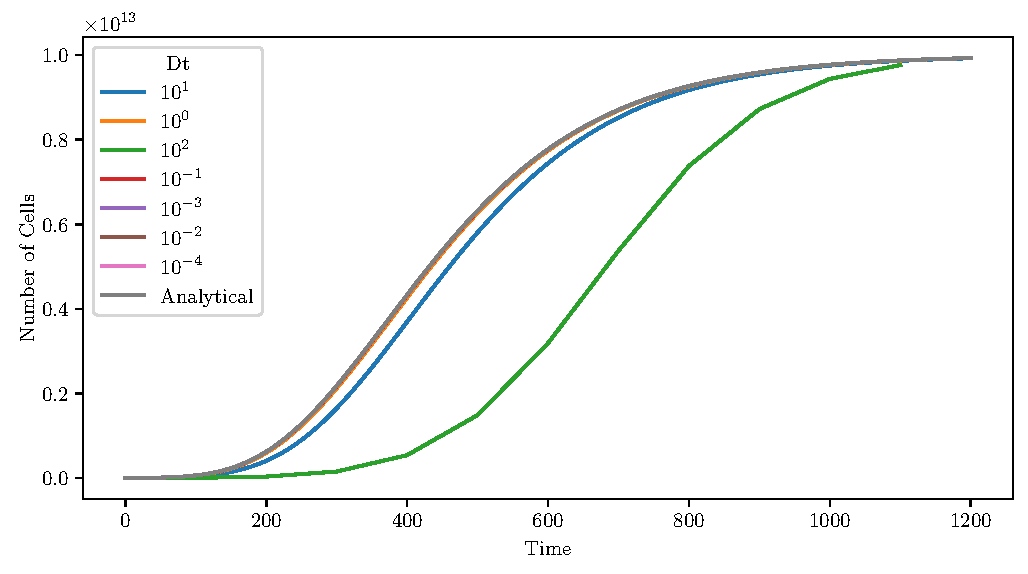
\includegraphics[width=14cm]{task2-1-h}
        \caption[Full simulation]{Full simulation}
        \label{fig:task2-1-h-full}
    \end{subfigure}

    \begin{subfigure}{\textwidth}
        \centering
        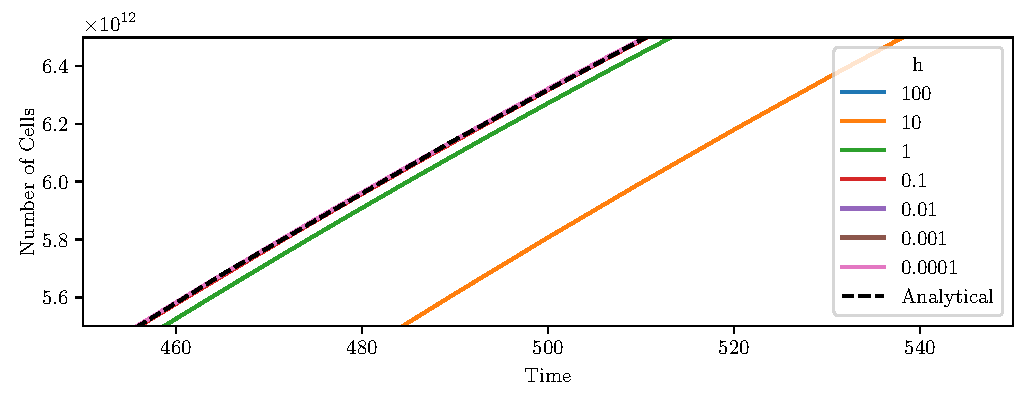
\includegraphics[width=14cm]{task2-1-h-zoom}
        \caption[Zoomed simulation]{Zoomed simulation}
        \label{fig:task2-1-h-zoom}
    \end{subfigure}
    \caption[Cell growth simulation with different dt values]{Cell growth simulation with different dt values}
    \label{fig:task2-1-h}
\end{figure}

The mean absolute percentage error for different values of $h$ relative to the analytical solution allows us to determine the optimal value of $h$ for the simulation.
Smaller values of $h$ result in a more accurate simulation, scaling linearly with the error as shown in \autoref{fig:task2-1-h-bar-error}.

\begin{figure}[!ht]
    \centering
    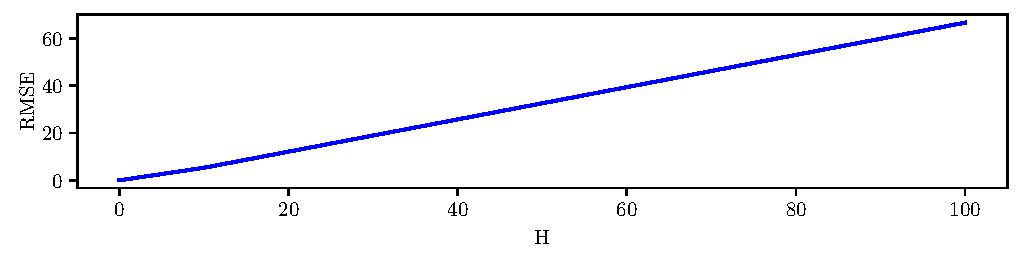
\includegraphics[width=14cm]{task2-1-h-bar-error}
    \caption[Cell growth simulation with different dt values (error)]{Cell growth simulation with different dt values (error)}
    \label{fig:task2-1-h-bar-error}
\end{figure}


% \begin{table}[ht]
%     \centering
%     \begin{tabular}{c | c} 
%         h & Error \\
%         \hline
%         100 & 66.69\% \\
%         10 & 5.296\% \\
%         1 & 0.5238\% \\
%         0.1 & 0.05233\% \\
%         0.01 & 0.005233\% \\
%         0.001 & 0.0005239\% \\
%         0.0001 & 5.82e-05\% \\
%         Analytical & 0.0 \\
%     \end{tabular}
%     \caption[Cell growth simulation error]{Cell growth simulation error}
% \end{table}

\clearpage

\subsection{Model Complexity}

The growth model is of $\bigO(n)$ complexity, where $n$ is the number of steps.
However, the value for $n$ is inversely proportional to the value of $h$ ($n = 1/h \times t$), 
smaller values of $h$ result in a longer computation time.

% Decreasing $h$ by a factor of 10 will increase the computation time by a factor of 10, this is a reciprocal relationship.

% So in terms of h and t, the relationship is linear.

\begin{figure}[ht]
    \centering
    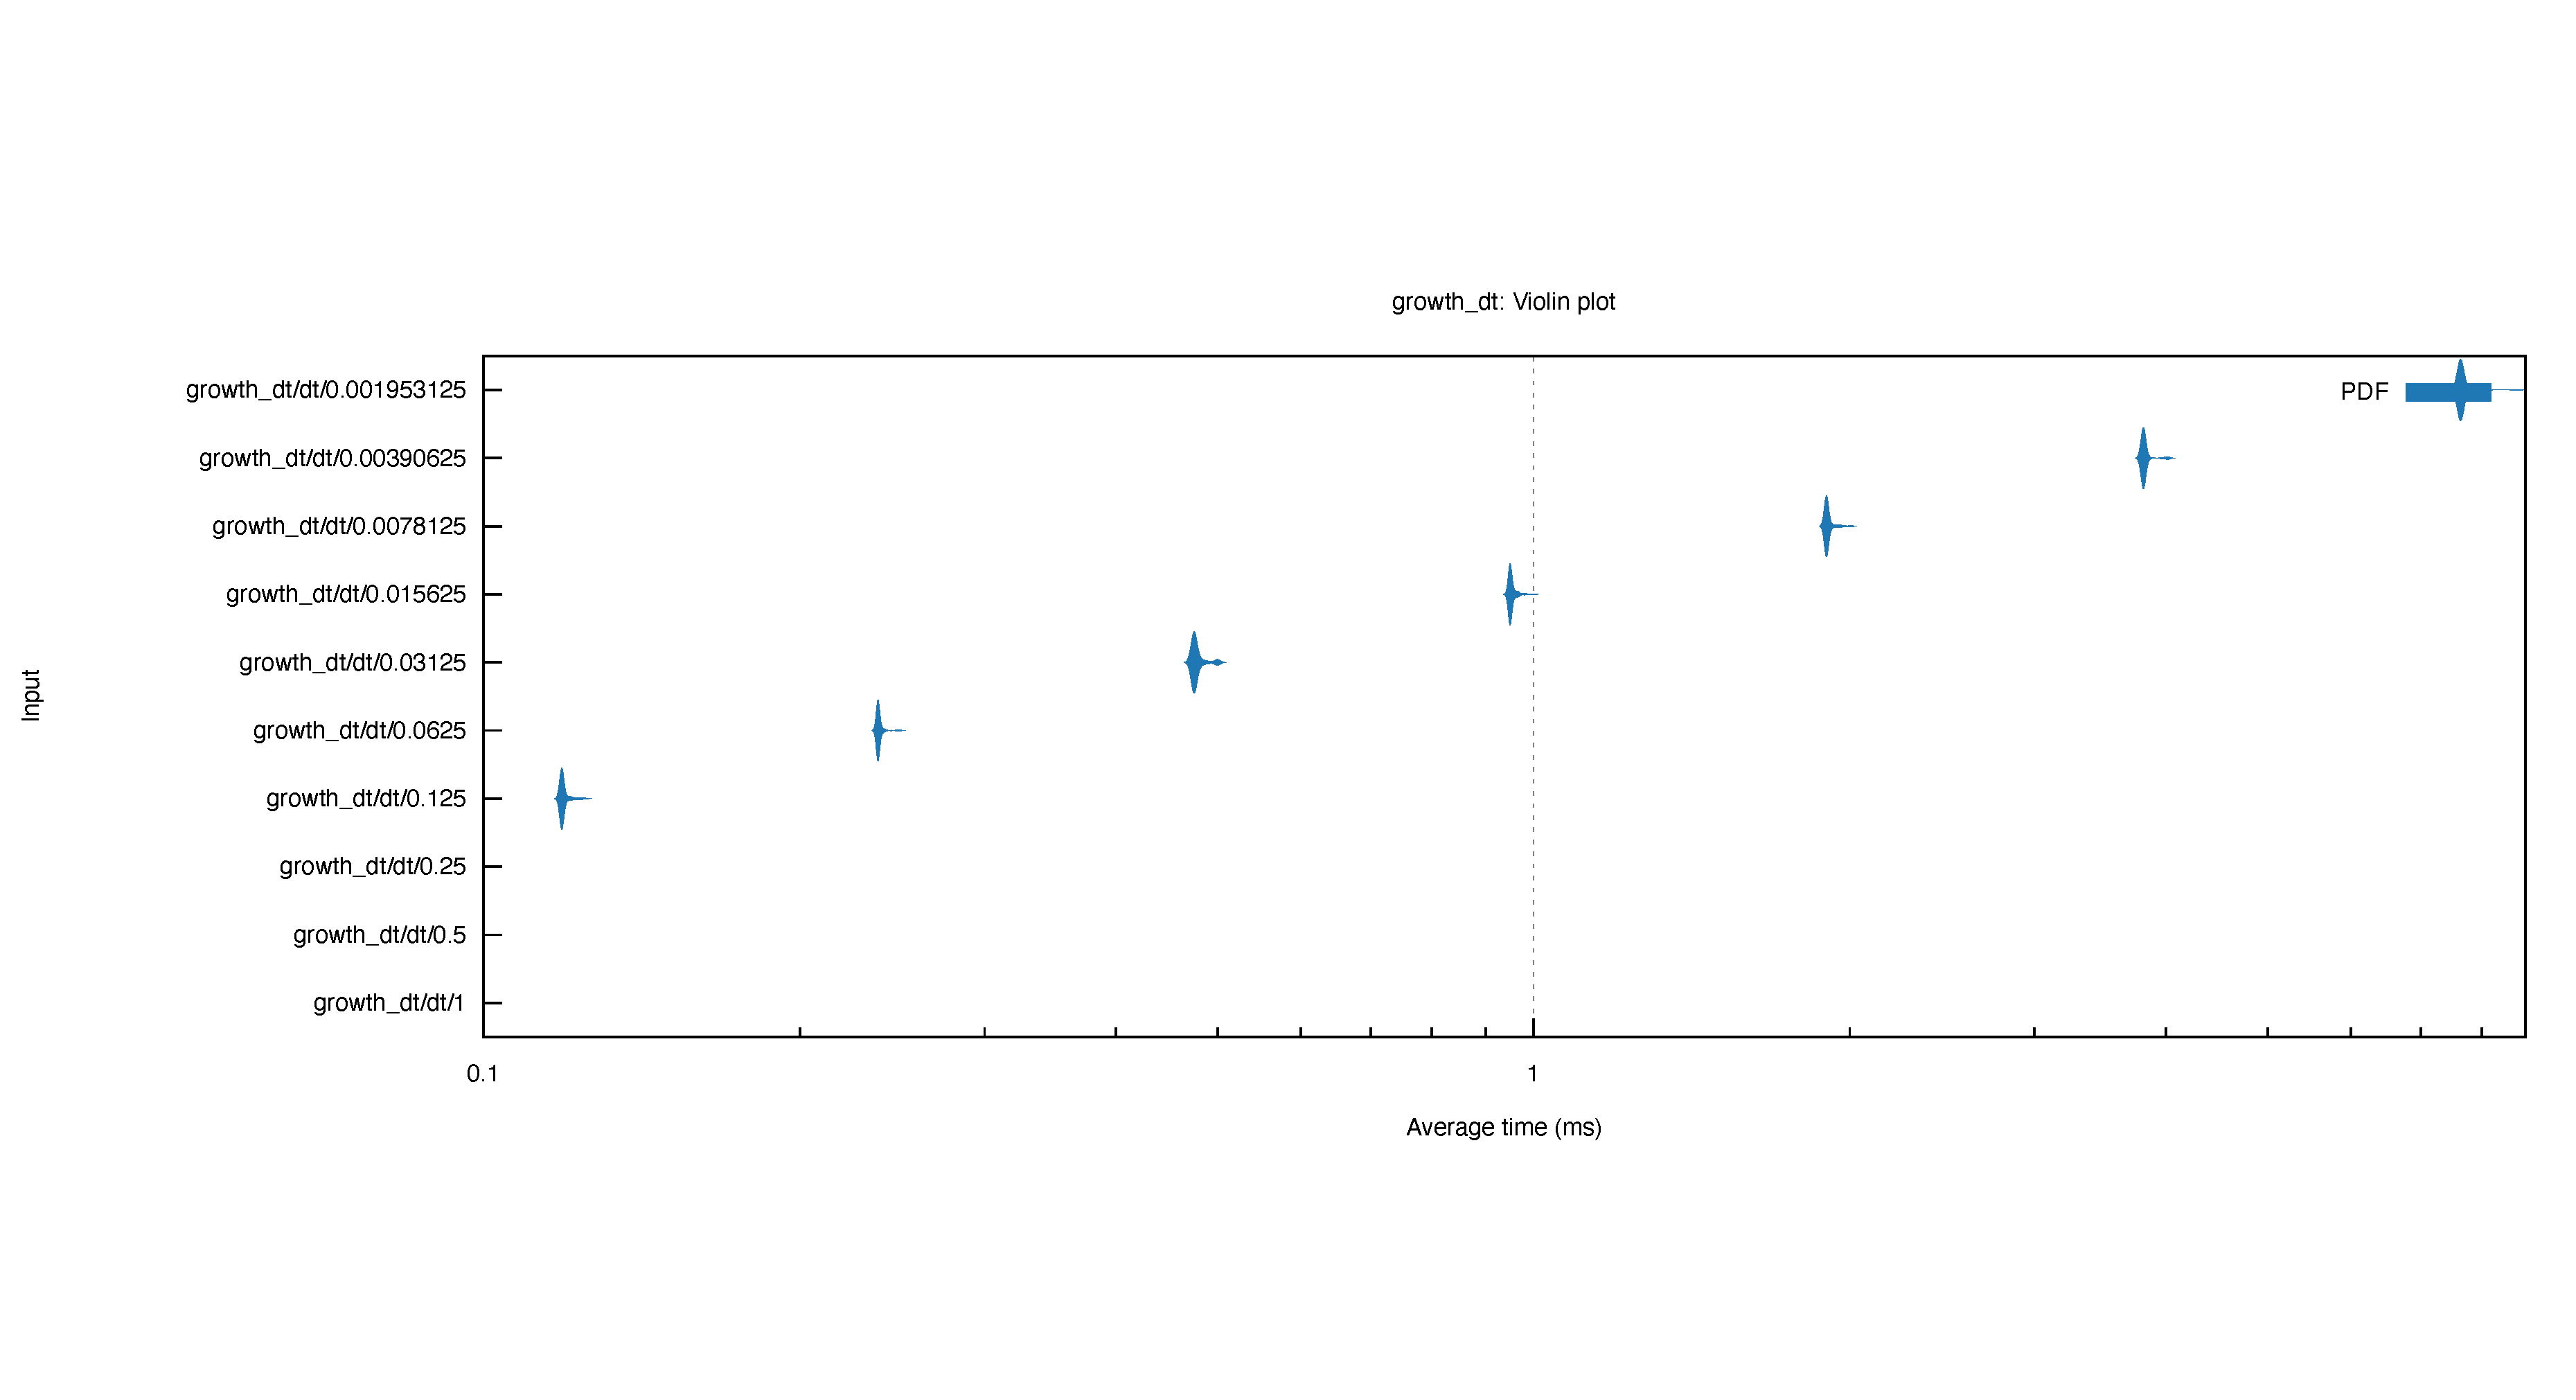
\includegraphics[width=\textwidth, clip, trim=4cm 6cm 1cm 8cm]{growth-dt-criterion}
    \caption[Cell growth criterion]{Cell growth criterion}
    \label{fig:growth-dt-criterion}
\end{figure}

\begin{figure}[ht]
    \centering
    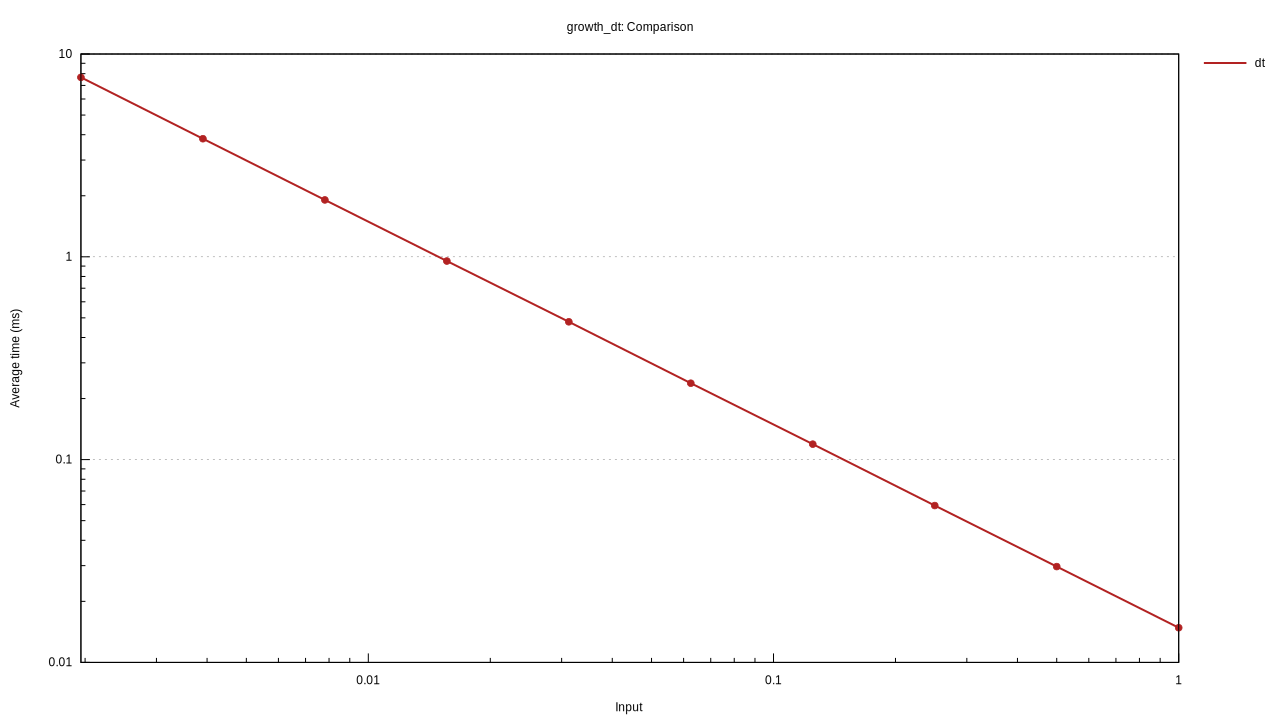
\includegraphics[width=\textwidth, clip, trim=1cm 0.1cm 5cm 2.2cm]{growth-dt-criterion-lines}
    \caption[Cell growth criterion (line)]{Cell growth criterion (line)}
    \label{fig:growth-dt-criterion-lines}
\end{figure}

By plotting both the value for $h$ and $t$ with logarithmic scales, the reciprocal relationship can be hidden.
Criterion benchmarks in \autoref{fig:growth-dt-criterion} and \autoref{fig:growth-dt-criterion-lines} show that growth is of $\bigO(n)$ complexity (linear).


\clearpage

\subsection{Changing the Capacity}

Changing the capacity value M for the differential equation will change the rate of growth proportionally, as shown in \autoref{fig:task2-1-m}. 

\begin{figure}[ht]
    \centering
    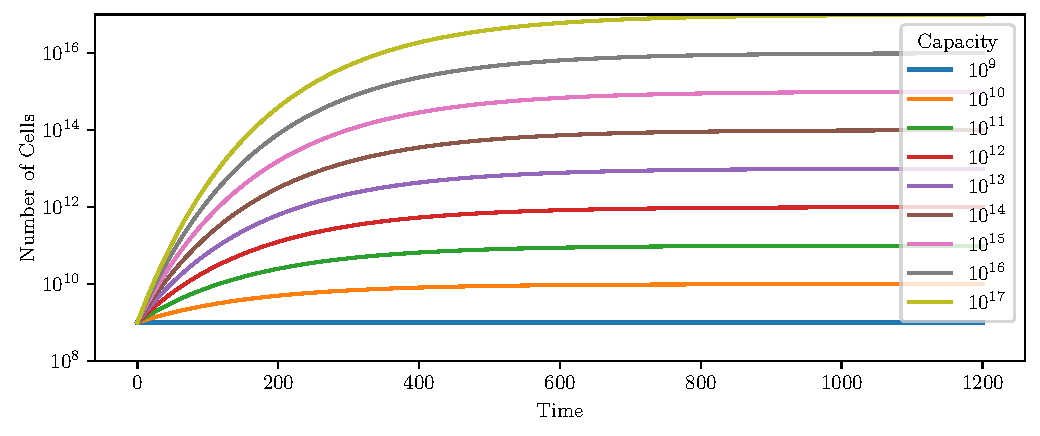
\includegraphics[width=14cm]{task2-1-m}
    \caption[Cell growth simulation with different capacity values]{Cell growth simulation with different capacity values}
    \label{fig:task2-1-m}
\end{figure}

However, this is not perfectly linear, as the rate of growth is logarithmic with respect to the capacity value $M$.
This is shown in \autoref{fig:task2-1-m-percent} with percentage values.

\begin{figure}[ht]
    \centering
    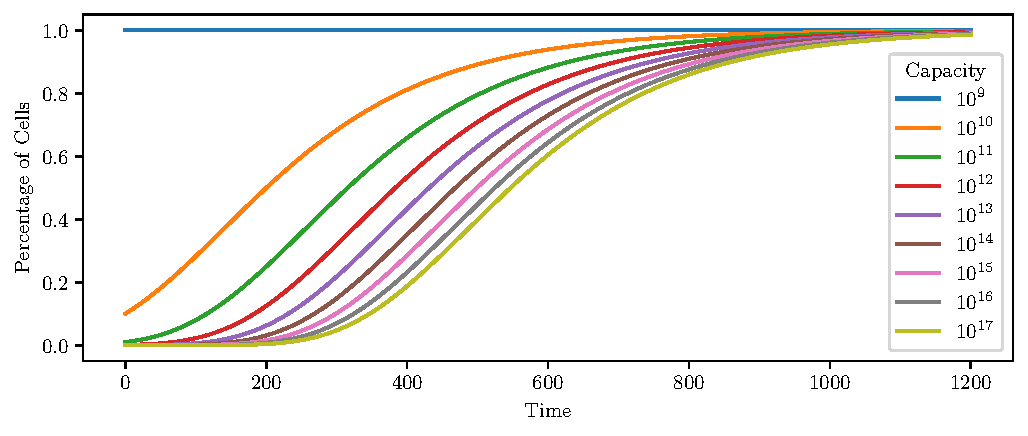
\includegraphics[width=14cm]{task2-1-m-percent}
    \caption[Cell growth simulation with different capacity values (percentage)]{Cell growth simulation with different capacity values (percentage)}
    \label{fig:task2-1-m-percent}
\end{figure}

\clearpage

% \[ \frac{dN}{dt}  = kNln\left(\frac{M}{n} \right) \]

% Increasing the value of M will increase the rate of growth.

% Different percentage of cells at the final time for different values of M.


While this difference is very likely the result of the differential equation itself, it is important to check if accuracy is maintained for different values of $M$.
\autoref{fig:task2-1-m-bar-error} displays that the error increases linearly with the value of $M$.
This is because the larger values of $M$ use more digits and \verb|float64| only has a precision of 15-16 decimal digits.
We can prove the percentage difference is due to the value of $M$ rather than computational error,
by plotting the percentage filled against the analytical solution (\autoref{fig:task2-1-m-bar-percentage}).

\begin{figure}[ht]
    \centering
    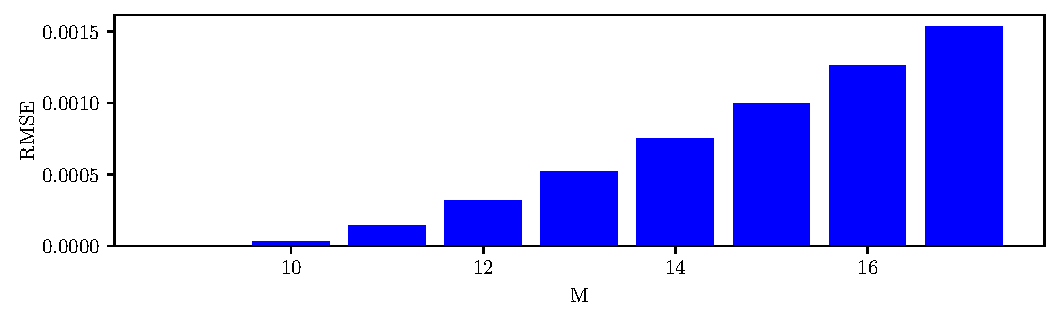
\includegraphics[width=14cm]{task2-1-m-bar-error}
    \caption[Cell growth simulation with different capacity values (error)]{Cell growth simulation with different capacity values (error) }
    \label{fig:task2-1-m-bar-error}
\end{figure}

\begin{figure}[ht]
    \centering
    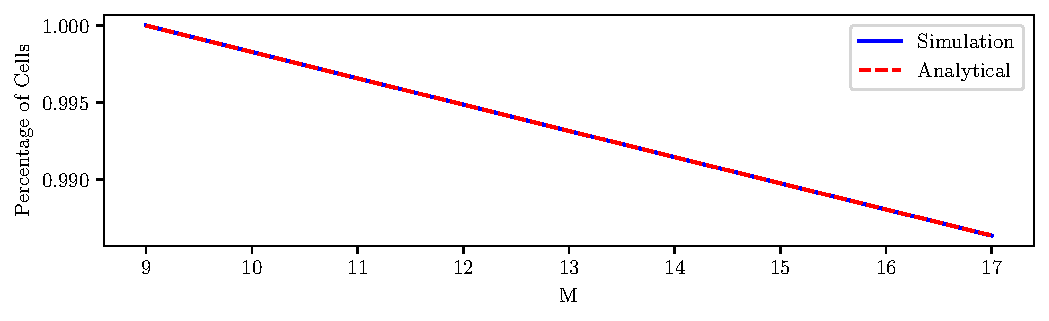
\includegraphics[width=14cm]{task2-1-m-bar-percentage}
    \caption[Cell growth simulation with different capacity values (percentage error)]{Cell growth simulation with different capacity values (percentage error) }
    \label{fig:task2-1-m-bar-percentage}
\end{figure}

The different values for $M$ do not significantly change the time to execute, as the resolution and time steps are the same (\autoref{fig:growth-m-criterion}).
This is not the case for $M=10^9$ as the initial capacity is $10^9$.
When performing the $dN/dt$ calculation, the result is zero.
Multiplications by zero are faster than multiplications by other values, hence the simulation is faster.

\begin{figure}[ht]
    \centering
    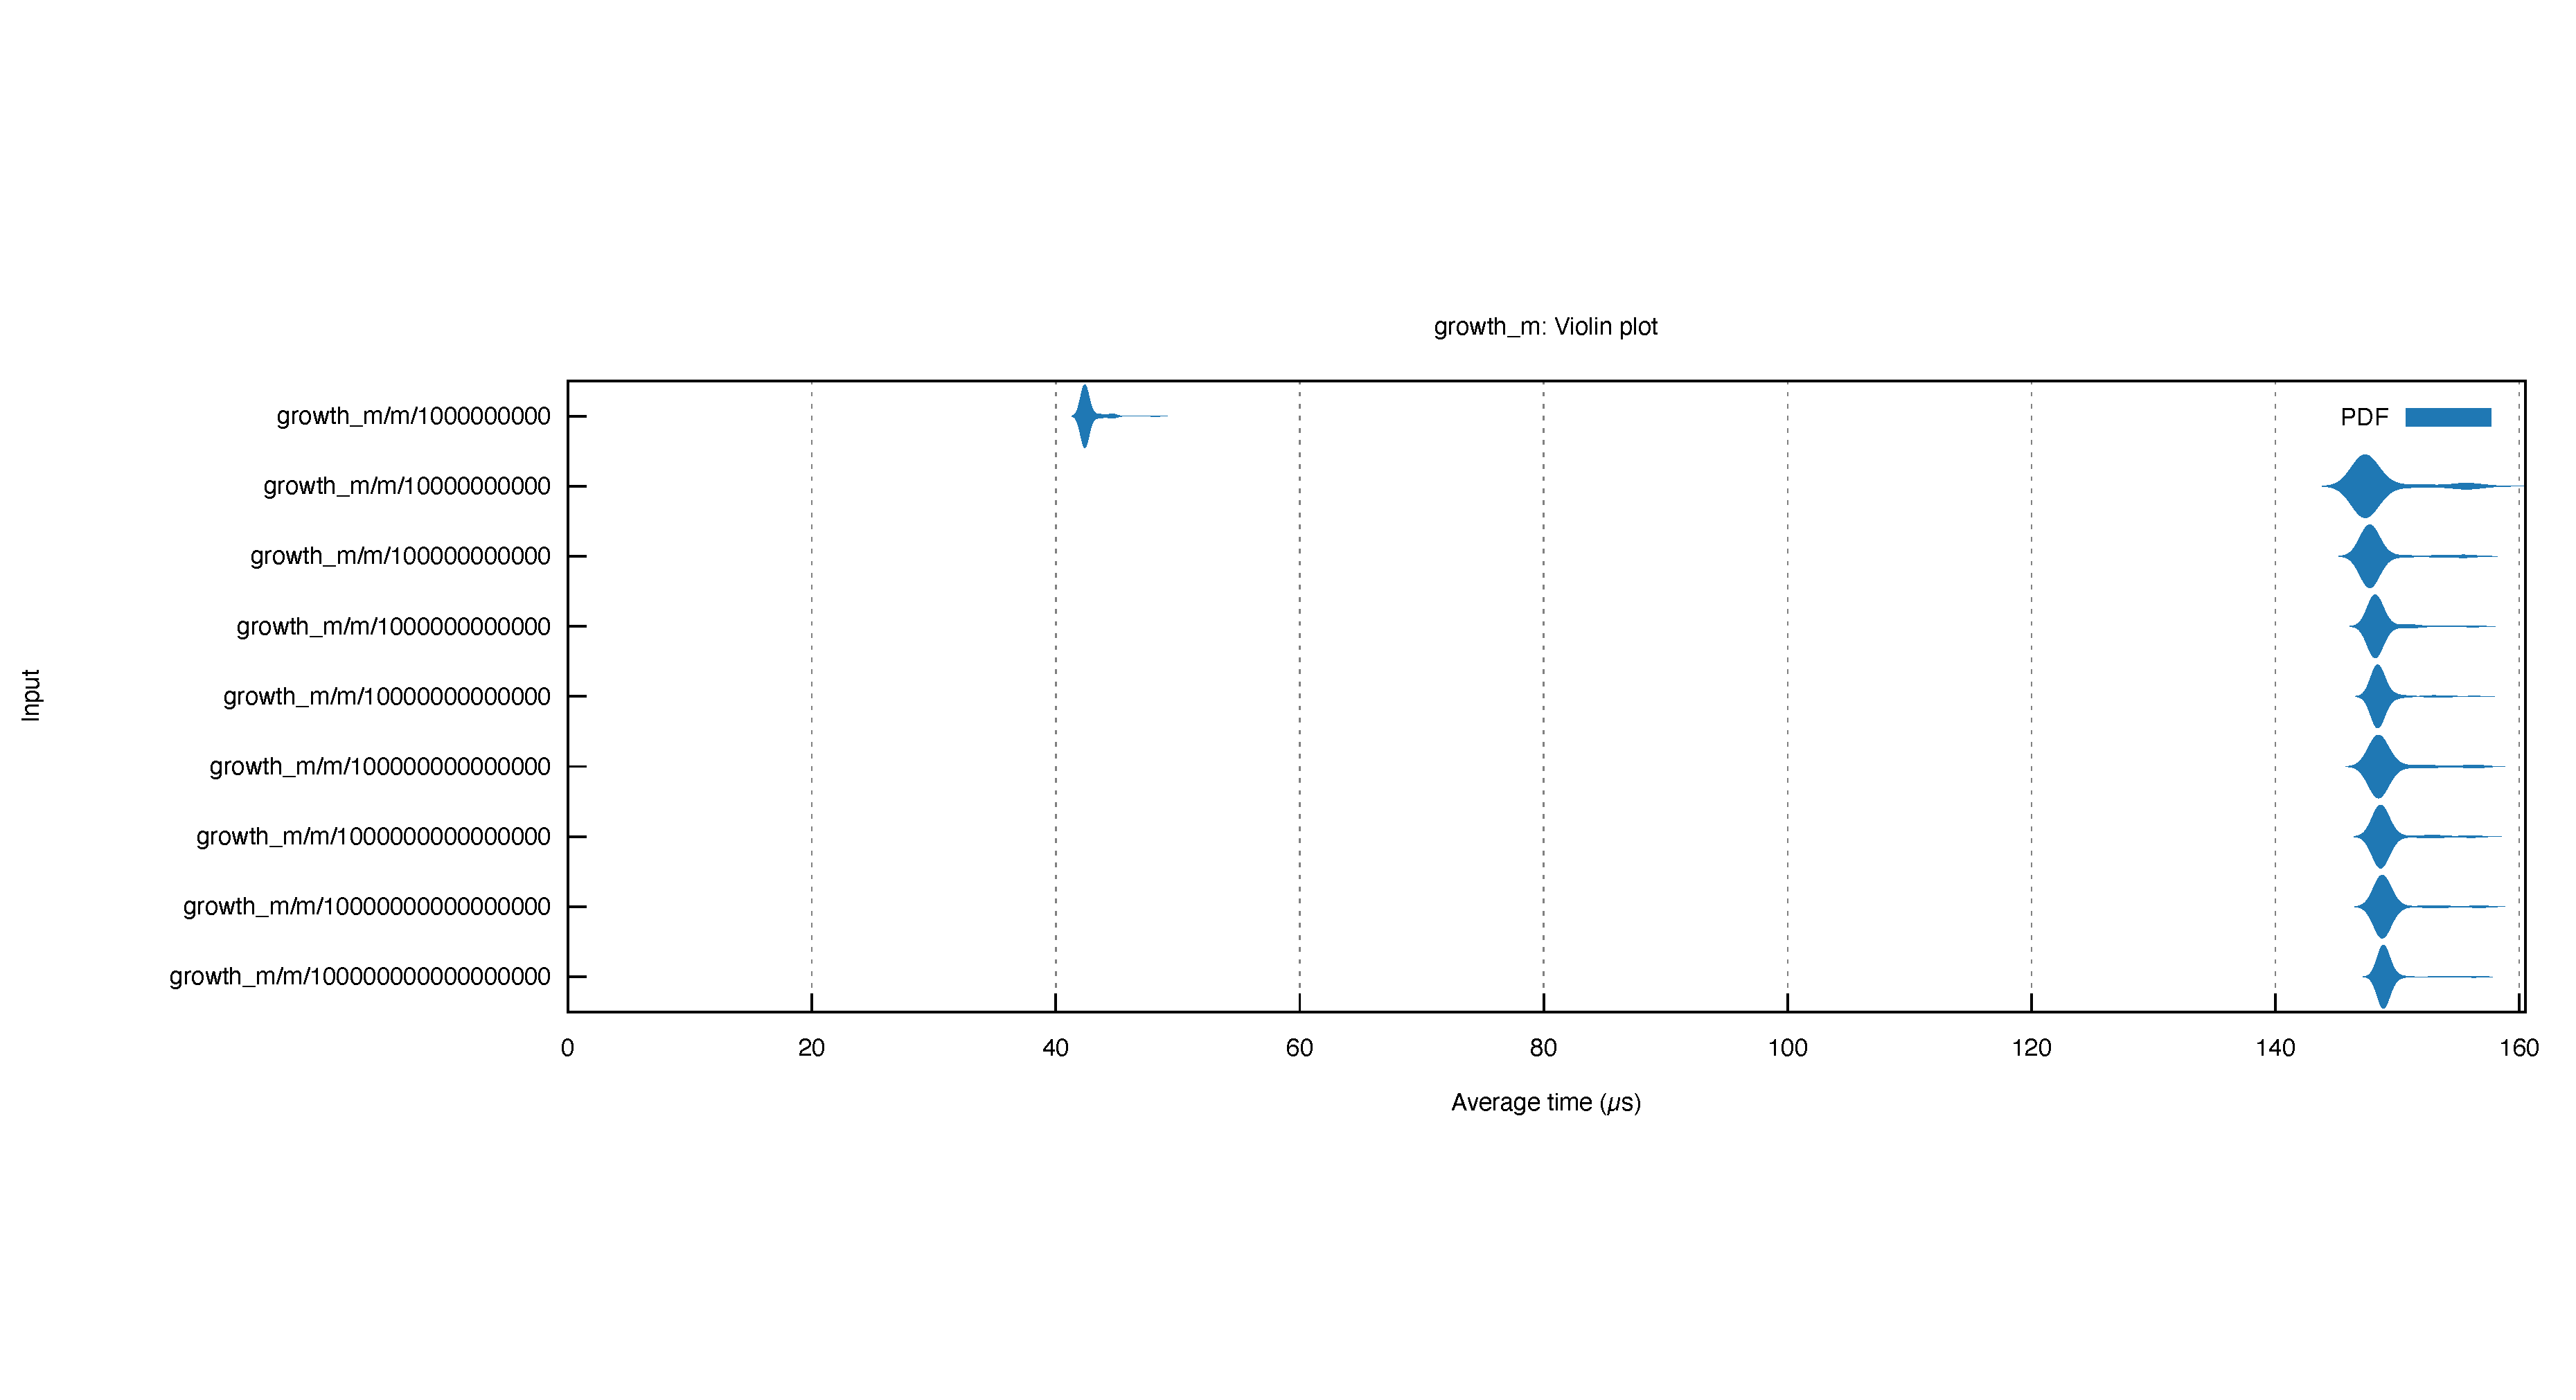
\includegraphics[width=\textwidth, clip, trim=4cm 6cm 1cm 8cm]{growth-m-criterion}
    \caption[Cell growth criterion ($M$)]{Cell growth criterion ($M$) }
    \label{fig:growth-m-criterion}
\end{figure}


\clearpage

\subsection{Random Walk}

Now we can take the random walk and apply it to the cell growth model to simulate the movement of cells within a tissue.
Before movement, the cells grow to a maximum capacity or a steady state. Once full, the cell moves in a random direction.
Given the random walk is independent of the growth model, we can expect the same results as the independent random walk, displayed in \autoref{fig:task2-2}.

\begin{figure}[ht]
    \centering
    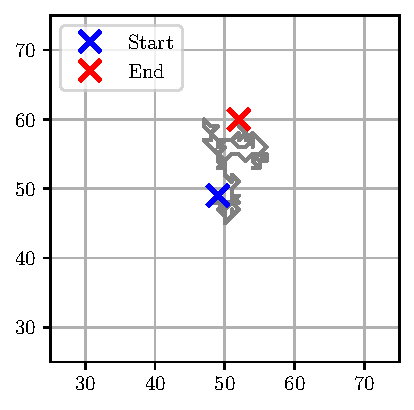
\includegraphics[width=5cm]{task2-2}
    \caption[Cell growth simulation with diagonal movement]{Cell growth simulation with diagonal movement}
    \label{fig:task2-2}
\end{figure}

When the random walk reaches a cell it has already visited, it will instantly move to a new cell as the percentage full will be already above the threshold.
Hence if the total number cells is plotted, we can expect a linear growth as shown in \autoref{fig:task2-2-total-linear} with 100 walk steps.
This linear growth can be estimated with a linear function at a steady state, until the tissue/grid is full.

% \begin{figure}[ht]
%     \centering
%     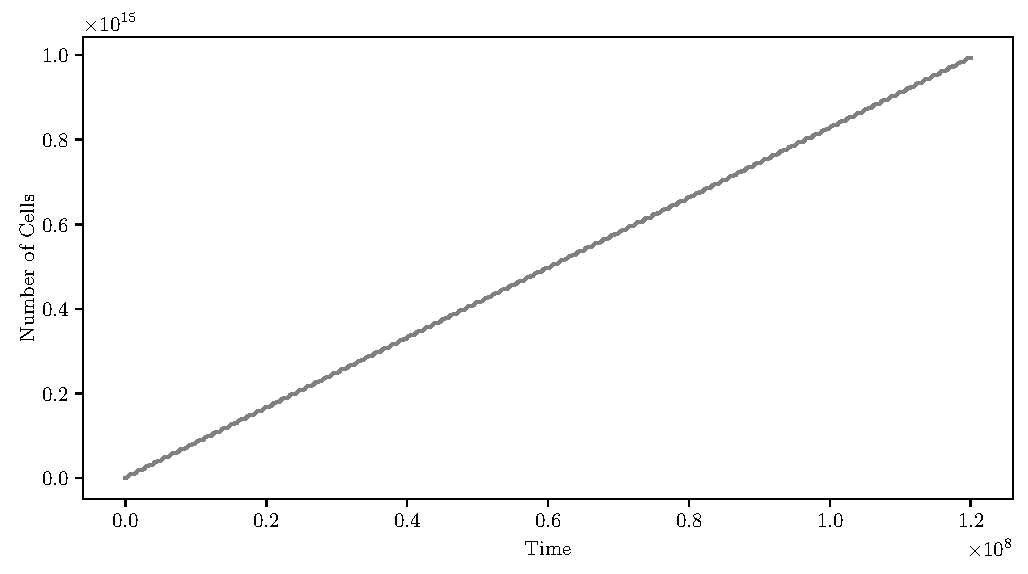
\includegraphics[width=14cm]{task2-2-total}
%     \caption[Cell growth simulation with diagonal movement (total cells)]{Cell growth simulation with diagonal movement (total cells)}
%     \label{fig:task2-2-total}
% \end{figure}

\begin{figure}[ht]
    \centering
    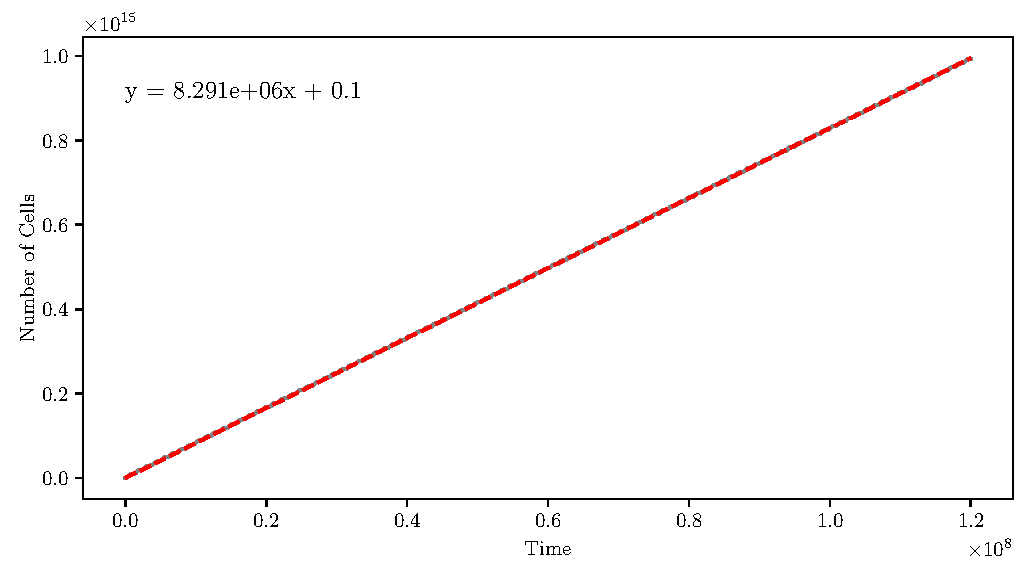
\includegraphics[width=14cm]{task2-2-total-linear}
    \caption[Cell growth simulation with diagonal movement (total cells) linear estimation]{Cell growth simulation with diagonal movement (total cells) linear estimation}
    \label{fig:task2-2-total-linear}
\end{figure}

\clearpage

\subsection{Changing the Grid Size}

All simulations to this point used a grid size of 100x100, with a maximum capacity of 10,000 cells areas.
\autoref{fig:task1-compare-grid} shows the simulations steps required to fill the grid for different grid sizes,
the graph is plotted against grid area.

\begin{figure}[ht]
    \centering
    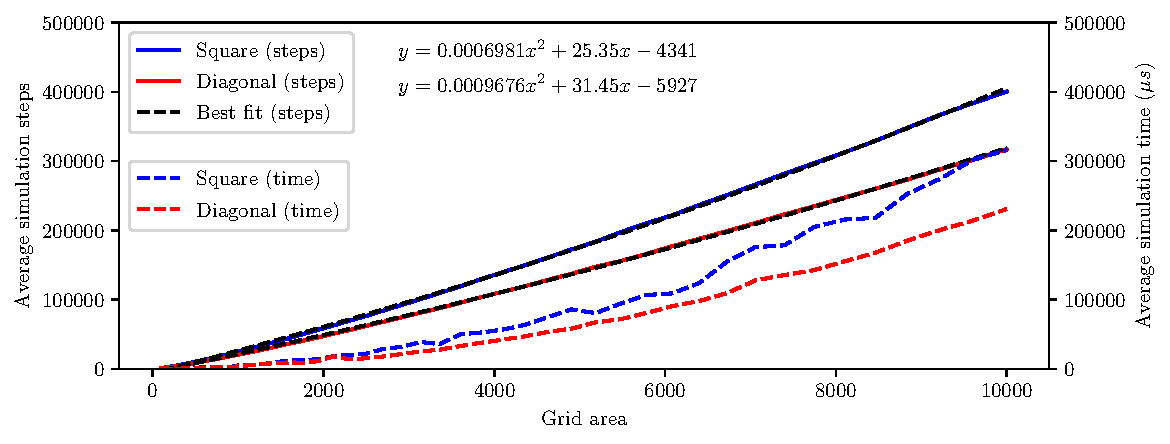
\includegraphics[width=14cm]{task1-compare-grid}
    \caption[Cell growth grid comparison]{Cell growth grid comparison}
    \label{fig:task1-compare-grid}
\end{figure}

The relationship between the grid area and the number of steps required to fill the grid is polynomial.
The growth model and random walk remain complexity of $\bigO(n)$ + $\bigO(n)$ = $\bigO(n)$,
however the grid size is now a factor in the complexity.
This added complexity is related to the concept of filling the grid and is of $\bigO(n^3)$ if $n$ is the grid width.